% questions.tex —— 1977 年·上海卷·理科 · 题目内容片段（无答案）
% 由 tools/generate_projects.py 依来源总账自 1977/1977_数学真题_上海理_试题.md 生成，勿手改（改源 MD 后重跑）


\begin{gktip}
\textbf{来源说明}：本题面依据固定源 PDF《1977 上海理科数学试题》第 1 页逐题转录。源文件为 A3 单页扫描，页脚印有“8”；原卷未附答案页。配套答案与解析为本库编者独立推导，\textbf{非官方标准答案}。第 9、10 题按原卷“附加题”保留在第 8 题之后，不计入正式题量。
\end{gktip}

\par\medskip

\begin{question}
\gkti{1}

\Needspace{5\baselineskip}
（1） 化简：

\nopagebreak[4]
\[
\left(\frac{a}{a+b}-\frac{a^2}{a^2+2ab+b^2}\right)\div\left(\frac{a}{a+b}-\frac{a^2}{a^2-b^2}\right).
\]

\Needspace{5\baselineskip}
（2） 计算：

\nopagebreak[4]
\[
\frac12\lg25+\lg2-\lg\sqrt{0.1}-\log_2 9\times\log_3 2.
\]

\Needspace{5\baselineskip}
（3） $\sqrt{-1}=i$，验算 $i$ 是否方程

\nopagebreak[4]
\[
2x^4+3x^3-3x^2+3x-5=0
\]

的解。

\Needspace{5\baselineskip}
（4） 求证：

\nopagebreak[4]
\[
\frac{\sin\left(\frac\pi4+\theta\right)}{\sin\left(\frac\pi4-\theta\right)}+\frac{\cos\left(\frac\pi4+\theta\right)}{\cos\left(\frac\pi4-\theta\right)}=\frac{2}{\cos2\theta}.
\]

\Needspace{0.4\textheight}
\end{question}
\begin{question}
\gkti{2}在 $\triangle ABC$ 中，$\angle C$ 的平分线交 $AB$ 于 $D$，过 $D$ 作 $BC$ 的平行线交 $AC$ 于 $E$，已知 $BC=a$，$AC=b$，求 $DE$ 的长。
\nopagebreak[4]
\begin{center}% 1977 年上海卷理科第 2 题：角平分线与平行线
\begin{tikzpicture}[scale=0.9]
  \coordinate (A) at (0,0);
  \coordinate (C) at (5,0);
  \coordinate (B) at (2.25,3.15);
  \coordinate (D) at ($(A)!0.43!(B)$);
  \coordinate (E) at ($(A)!0.43!(C)$);
  \draw[thick] (A)--(B)--(C)--cycle;
  \draw[thick] (D)--(C);
  \draw[thick] (D)--(E);
  \fill (A) circle (1.2pt) node[below left] {$A$};
  \fill (B) circle (1.2pt) node[above] {$B$};
  \fill (C) circle (1.2pt) node[below right] {$C$};
  \fill (D) circle (1.2pt) node[left] {$D$};
  \fill (E) circle (1.2pt) node[below] {$E$};
\end{tikzpicture}
\end{center}
\nopagebreak[4]
\end{question}
\begin{question}
\gkti{3}已知圆 $A$ 的直径为 $2\sqrt3$，圆 $B$ 的直径为 $4-2\sqrt3$，圆 $C$ 的直径为 $2$，圆 $A$ 与圆 $B$ 外切，圆 $A$ 又与圆 $C$ 外切，$\angle A=60^\circ$，求 $BC$ 及 $\angle C$。

\end{question}
\begin{question}
\gkti{4}正六棱锥 $V-ABCDEF$ 的高为 $2\ \mathrm{cm}$，底面边长为 $2\ \mathrm{cm}$。

（1） 按 $1:1$ 画出它的二视图；

（2） 求其侧面积；

（3） 求它的侧棱和底面的夹角。

\end{question}
\begin{question}
\gkti{5}解不等式：

\nopagebreak[4]
\[
\begin{cases}
16-x^2\geqslant0,\\
x^2-x-6>0,
\end{cases}
\]

并在数轴上把它的解表示出来。

\end{question}
\begin{question}
\gkti{6}已知两定点 $A(-4,0)$、$B(4,0)$，一动点 $P(x,y)$ 与两定点 $A\text{、}B$ 的连线 $PA\text{、}PB$ 的斜率的乘积为 $-\dfrac14$。求点 $P$ 的轨迹方程，并把它化为标准方程，指出是什么曲线。

\Needspace{0.4\textheight}
\end{question}
\begin{question}
\gkti{7}等腰梯形的周长为 $60$，底角为 $60^\circ$，问这梯形各边长为多少时，面积最大？
\nopagebreak[4]
\begin{center}% 1977 年上海卷理科第 7 题：等腰梯形
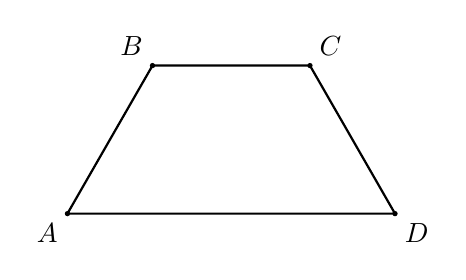
\begin{tikzpicture}[scale=0.8]
  \coordinate (A) at (0,0);
  \coordinate (D) at (5.2,0);
  \coordinate (B) at (1.35,2.35);
  \coordinate (C) at (3.85,2.35);
  \draw[thick] (A)--(B)--(C)--(D)--cycle;
  \fill (A) circle (1.2pt) node[below left] {$A$};
  \fill (B) circle (1.2pt) node[above left] {$B$};
  \fill (C) circle (1.2pt) node[above right] {$C$};
  \fill (D) circle (1.2pt) node[below right] {$D$};
\end{tikzpicture}
\end{center}
\nopagebreak[4]
\Needspace{0.4\textheight}
\end{question}
\begin{question}
\gkti{8}当 $k$ 为何值时，方程组

\nopagebreak[4]
\[
\left\{
\begin{aligned}
x-\sqrt{y-2}&=0 &&(1),\\
kx-y-2k-10&=0 &&(2)
\end{aligned}
\right.
\]

有两组相同的解？并求出它的解。

\begin{gktip}
\Needspace{0.25\textheight}
\textbf{附加题}
\end{gktip}

\textbf{附加题 9．} 如图所示，半圆 $O$ 的直径为 $2$，$A$ 为半圆直径的延长线上的一点，且 $OA=2$，$B$ 为半圆上任一点，以 $AB$ 为边作等边 $\triangle ABC$，问 $B$ 在什么地方时，四边形 $OACB$ 的面积最大？并求出这个面积的最大值。
\nopagebreak[4]
\begin{center}% 1977 年上海卷理科附加题：半圆与等边三角形
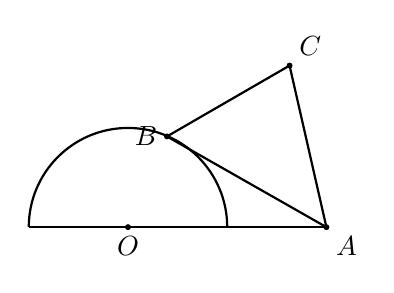
\begin{tikzpicture}[scale=0.9]
  \coordinate (O) at (0,0);
  \coordinate (L) at (-1.4,0);
  \coordinate (R) at (1.4,0);
  \coordinate (A) at (2.8,0);
  \coordinate (B) at (0.55,1.28);
  \coordinate (C) at (2.28,2.28);
  \draw[thick] (L) arc (180:0:1.4);
  \draw[thick] (L)--(A);
  \draw[thick] (B)--(A)--(C)--cycle;
  \fill (O) circle (1.2pt) node[below] {$O$};
  \fill (A) circle (1.2pt) node[below right] {$A$};
  \fill (B) circle (1.2pt) node[left] {$B$};
  \fill (C) circle (1.2pt) node[above right] {$C$};
  \draw[dashed] (O)--(A);
\end{tikzpicture}
\end{center}
\nopagebreak[4]
\textbf{附加题 10．} 已知曲线 $y=x^2-2x+3$ 与直线 $y=x+3$ 相交于点 $P(0,3)\text{、}Q(3,6)$ 两点。

\begin{itemize}
\item \textbf{（1）} 分别求出曲线在交点的切线的斜率；
\end{itemize}

\begin{itemize}
\item \textbf{（2）} 求出曲线与直线所围成的图形的面积。
\end{itemize}

\end{question}